\documentclass[12pt, letterpaper]{article}
\usepackage[utf8]{inputenc}
 \usepackage[letterpaper, margin=1in]{geometry}
 \usepackage{amssymb}
\usepackage{amsmath}
 \usepackage{enumitem}
\usepackage {listings}
\usepackage{pgfplots}
\usepgfplotslibrary{external}
\usepackage{graphicx}

\title{CS425 Project1 (Report)\\Multiple Linear Regression Analysis}
\author{Ksenia Burova}
\date{October \(1^{st}\), 2017}

\begin{document}
\maketitle

\noindent {\bf Abstract:} In machine learning, multiple regression is a function if multiple inputs (discrete or numeric), that has one output that is a class code or continuous value. \\
In this project, the goal was to predict the gas milage of automobiles from their other multiple attributes by using multiple linear regression. We were given two files, one with data and another one with attribute information for that data. Six values for horsepower were missing, and had to be skipped or predicted. Data attributes contained both, discrete and numeric values. We had to compare performance of data with and without standardization. After calculating weights, we had to analyze which attribute was the best in predicting gas milage. 

\begin{enumerate}[label=\Roman*.]
	
	{\bf \item Project data} \\
	
	The following attributes are provided:
	\begin{itemize}
		\item    mpg:           continuous  -  {\bf to be predicted}
		\item    cylinders:     multi-valued discrete
		\item    displacement:  continuous
		\item    horsepower:    continuous
		\item    weight:        continuous
		\item    acceleration:  continuous
		\item    model year:    multi-valued discrete
		\item    origin:        multi-valued discrete
		\item    car name:      string (unique for each instance) - {\bf not used}
	\end{itemize}
	
	We represent data ( all but milage and names) in a matrix form:\\
	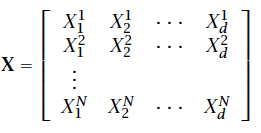
\includegraphics[scale=0.5]{pics/matrix.png} \\
	
	Each column is a single attribute, each row is a single experiment or data sample (in our case, all params for one unique car).
	
	{\bf \item Resolving missing values} \\
	
	There are six observations where horsepower attribute is not defined. Sometimes it is the best strategy to discard those observations. Another way is  to estimate those values using {\it imputation} method. There is mean imputation and imputation by regression possible. \\
	I've used two approaches: ignored observations with missing values and I tried mean imputation. 
	
	{\bf \item Calculating weights with Multiple Regression} \\
	(Equations are copied from the textbook) \\
	
	Going back to multiple regression, our numeric output is vector {\it r} which represents milage attribute.  We have a weighted sum of attributes \( x_1, x_2 ... x_d\) and some noise.  \\
	
	Here is a multivariate linear model: \\
	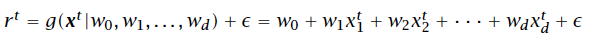
\includegraphics[scale=0.5]{pics/model.png} \\
	We may assume error to be normal with mean 0 and constant variance. To maximize the likelihood we will minimize the sum of squared errors: \\
	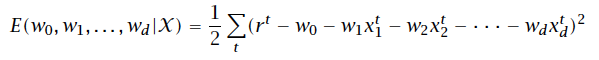
\includegraphics[scale=0.5]{pics/errors.png} \\
	Taking derivative with respect to parameters we get the normal equations: \\
	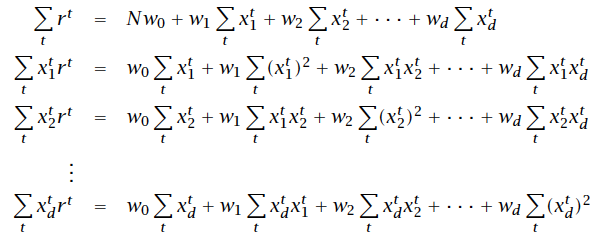
\includegraphics[scale=0.5]{pics/normal.png} \\
	We now can define the matrix of attributes (as before) but with first column being all ones, since in our model \(w_0\) term is the same as \(w_0 \cdot 1 \). We can define a vector of all weights, and an output vector which is our milage values. So we get: \\
	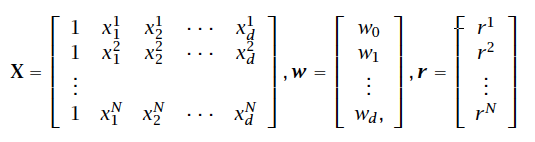
\includegraphics[scale=0.5]{pics/attr.png} \\ 
	Then the normal equations can be written this way now: \\
	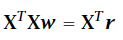
\includegraphics[scale=0.5]{pics/eq.png} \\
	And we can derive weights: \\
	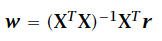
\includegraphics[scale=0.5]{pics/weights.png} \\
	So the goal is to compute and analyze these weights.
	
	{\bf \item Program structure} \\\\
	I've written my application in Python as was suggested. I've used {\it numpy} library to use matrix operations on vectors. \\
	I have two files.  I've defined a class {\it MultRegression} in one and have written functions for calculating mean, standard deviation, data standardization and weights. My second one is basically like main, I create an instance of the class and pass parameters.\\
	I pass 3 parameters to my class (I manually modify them in main function): 
	\begin{enumerate}[label=\arabic*.]
		\item Data file name 'auto-mpg.data'
		\item Boolean value to decide if i need to standardize my data. 1 - yes, 0 - no
		\item Boolean value to decide if I need to skip data with missing attributes. 1 - yes, 0 - no
	\end{enumerate}
	I've tested my functions on smaller data examples and matrices before running it on givven data.
	
	{\bf \item Results} \\
	
	The first time I ran my program I skipped lines with missing attributes and I didn't standardize parameters. I received following values for weights:
	\begin{verbatim}
	[ -1.80586717e+01  -4.18254893e-01   1.88870416e-02  -1.13851962e-02
  	-6.71865820e-03    1.02620868e-01   7.56755050e-01   1.41751561e+00]
	\end{verbatim}
	It is really hard to analyze these values since attributes that were expected to have negative effect on milage have a corresponding weight with positive sign, like car displacement. More horsepower and cylinders do have a negative effect on milage, as expected. It is hard to analyze absolute values though. \\
	Usually data standardization is needed when we use attributes of different types that have different value ranges. Here are results after standardization:
	\begin{verbatim}
	[ 20.37880831  -5.00325077  -2.37809451  -0.7357686    
	 2.30248253     0.4401979     3.09178799   6.02984611]
	\end{verbatim}
	We can see that number of cylinders, car displacement and horsepower have negative effects on gas milage, as expected. Where other attributes have a more positive effect. it is possible, that newer car would have greater gas milage, so results look fine so far.
	Now, I estimated horsepower for samples with missing values and added those:
	\begin{verbatim}
	[ 20.36175876  -4.70649111  -3.1073928   -0.05821537
	   1.98385778   0.43863716   2.88210938   6.30068179]
	\end{verbatim}
	The absolute values have changed, looking at absolute values of weights corresponding to horsepower we can assume now that that attribute is almost useless in predicting milage, which can't be really true. So sometimes, it is better to remove values from data than estimate values that may influence results in negative way. Or maybe better predicting algorithm should be used like imputation by regression to get better estimated values with less noise.
	
	Now let's look at plots for given data: \\
	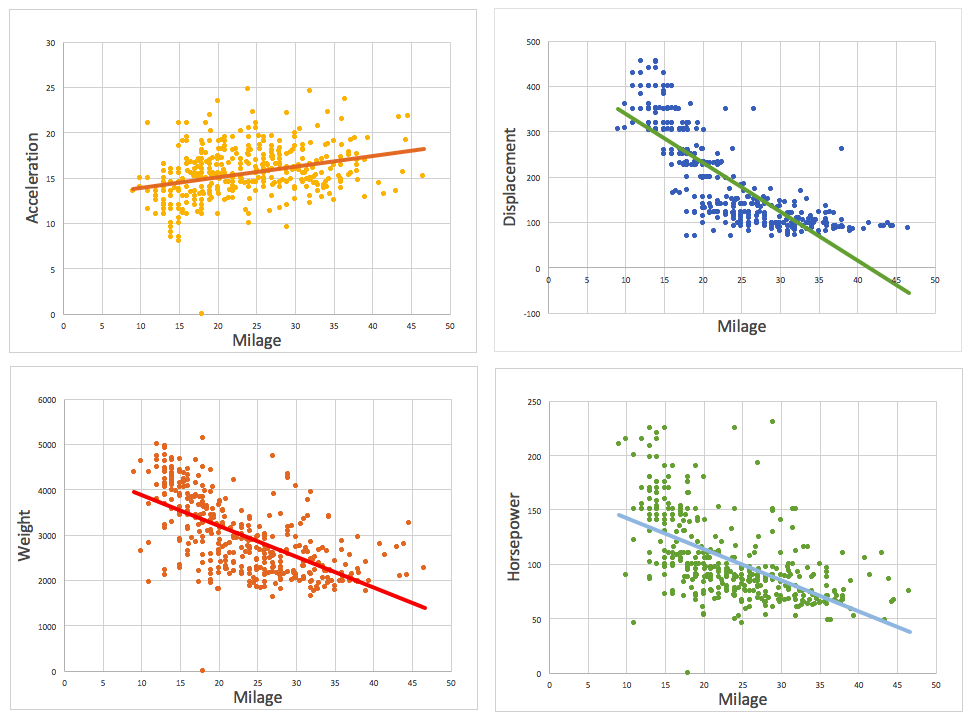
\includegraphics[scale=0.45]{pics/contplots.png} \\
	
\end{enumerate}
	
\end{document} 